% !TEX encoding = UTF-8 Unicode

\documentclass[a4paper]{article}

\usepackage{color}
\usepackage{listings}
\usepackage{url}
\usepackage[T2A]{fontenc} % enable Cyrillic fonts
\usepackage[utf8]{inputenc} % make weird characters work
\usepackage{graphicx}
\usepackage{verbatim}

\usepackage[english,serbian]{babel}
%\usepackage[english,serbianc]{babel} %ukljuciti babel sa ovim opcijama, umesto gornjim, ukoliko se koristi cirilica

\usepackage[unicode]{hyperref}
\hypersetup{colorlinks,citecolor=green,filecolor=green,linkcolor=blue,urlcolor=blue}

%\newtheorem{primer}{Пример}[section] %ćirilični primer
\newtheorem{primer}{Primer}[section]

\begin{document}

\title{Uvod u programiranje\\ \small{Skipta za kurs\\Uvod u programiranje kroz JavaScript\\}}

\author{Una Stanković\\ una.stankovic@code.edu.rs}
\date{10.~septembar 2018.}
\maketitle
\newpage

U ovom tekstu predstavljene su teorijske osnove potrebne za savladavanje kursa $"$ Uvod u programiranje kroz JavaScript$"$. Najpre su navedene, ukratko, teorijske osnove računarstva i uvod kroz HTML i CSS, a kasnije se ulazi u rad sa JavaScript-om.  Ova skripta je obavezan materijal pri kursu i sa prezentacijama i kodovima formira celinu. Ova skripta sama po sebi nije dovoljna, samostalan rad i istraživanje je neizostavni deo procesa učenja. U slučaju da primetite greške pri čitanju rada ili imate bilo kakve nedoumice, predloge i sugestije javite se mejlom na adresu navedenu na prvoj strani.

\newpage

\tableofcontents

\newpage

\section{Uvod u računarstvo}
\label{sec:uvod}
Računarstvo i informatika predstavljaju jednu od najvažnijih oblasti današnjice koje su u konstantnom razvoju. Danas, ne možemo zamisliti život bez računara, pametnih telefona ili mnogobrojnih uređaja koji se pokreću uz pomoć računara. Razvitak računarstva i tehnologije u poslednjih 70 godina je eksponencijalan, tako da, danas, imamo razvoj prenosnih računara, tableta, pametnih telefona i uređaja, kola, kućnih aparata i ostalih koji se pokreću korišćenjem računarskih sistema. Kako definisati računarski sistem? Postoji više različitih računarskih sistema, od kojih svaki ima svoju posebnu definiciju, ali naš fokus je na digitalnim računarskim sistemima. Oni podrazumevaju mašinu koja može da se programira kako bi izvršavala različite zadatke svođenjem na elementarne operacije nad brojevima. Brojevi se u računaru zapisuju uz pomoć nula i jedinica, odnosno, binarnim zapisom, kao nizovi bitova. \\\\
Kada se razmišlja o tome šta sve računarstvo obuhvata, lako se uviđa da računarstvo nije samo računar, već da ono predstavlja mnogo širu oblast koja se bavi izučavanjem teorije i prakse procesa računanja i primene računara u različitim naučnim oblastima, tehnici i svakodnevnom životu. Računar sam po sebi nije cilj, već sredstvo za postizanje različitih ciljeva u zavisnosti od njihove primene. Za današnje računare često ćemo čuti da su $"$programabilni$"$, ali šta to zapravo govori? Programabilnost računara se ogleda u činjenici da je moguće računaru dati neki skup instrukcija koje će on izvršavati sa ciljem ispunjavanja određenih zadataka, koje mu čovek, odnosno, programer zadaje. Računari kakve danas poznajemo nastali su polovinom XX veka, ali želja za automatizacijom određenih postupaka seže daleko dalje u prošlost. Naime, posmatrajući istorijski, ljudi su vekovima stvarali razne naprave koje su mogle da rešavaju neke numeričke zadatke. 

\subsection{Istorijat računarstva}
Da bismo u potpunosti razumeli računarstvo moramo imati uvid u njegove početke i razvoj. Istorijski gledano, koreni ljudske želje da olakšaju sebi svakodnevni život sežu davno u prošlost. Kao pravi primer takvih težnji možemo uzeti jedne od prvih računaljki abakus. U $18.$ veku nastale su prve mehaničke sprave koje su mogle da vrše automatsko izvođenje aritmetičkih operacija i pomažu u rešavanju matematičkih zadataka. Blez Paksal\footnote{Blaise Pascal (1623–1662), francuski filozof, matematičar i fizičar. U njegovu čast jedan
programski jezik nosi ime PASCAL.} je $1642.$ godine konstruisao mehaničke sprave koje su služile za sabiranje i oduzimanje celih brojeva, zvane Paskaline. Trideset godina nakon njega, Godfrid Lajbnic\footnote{Gottfried Wilhelm Leibniz (1646–1716), nemački filozof i matematičar} konstruisao je mašinu, zasnovanu na dekadnom sistemu, koja je mogla da vrši sve četiri osnovne operacije. Lajbnic je bio prvi koji je predlagao koriscenje binarnog sistema.\\\\ 
\begin{figure}[h!]
\begin{center}
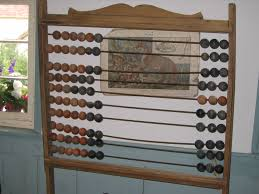
\includegraphics[scale=0.5]{pictures/abakus.jpg}
\end{center}
\caption{Abakus}
\label{fig:abakus}
\end{figure}
\begin{figure}[h!]
\begin{center}
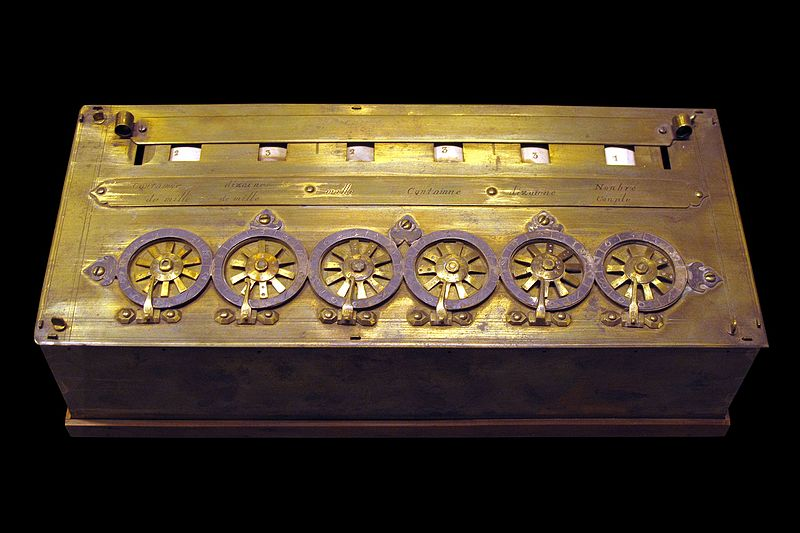
\includegraphics[scale=0.25]{pictures/pasc.jpg}
\end{center}
\caption{Paskalina}
\label{fig:pasc}
\end{figure}
\subparagraph{Mehaničke mašine} Žozef Mari Žakard\footnote{Joseph Marie Jacquard (1752–1834), francuski trgovac.} je $1801.$ godine napravio prvu programabilnu mašinu — mehanički tkački razboj. On je pomoću bušenih kartica
kreirao kompleksne šare na tkanini. Svaka rupa na kartici određivala je jedan pokret mašine, a svaki red na kartici odgovarao je jednom redu šare.
\begin{figure}[h!]
\begin{center}
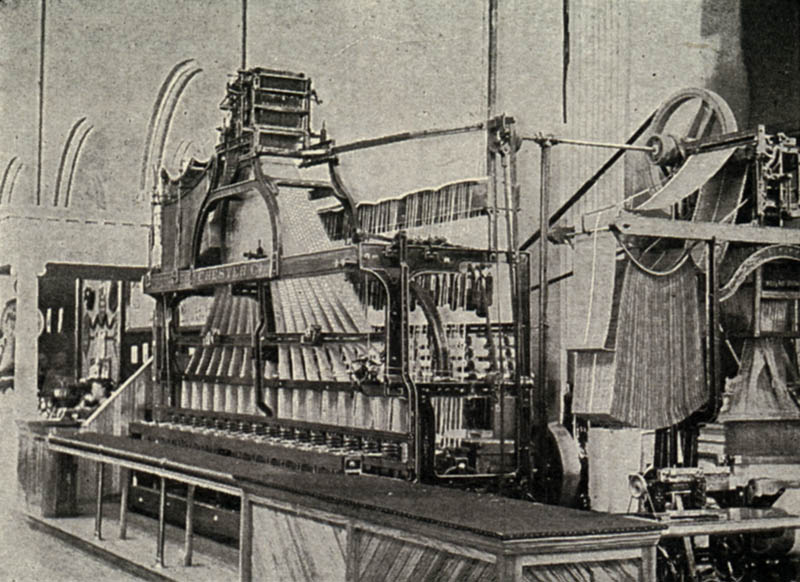
\includegraphics[scale=0.25]{pictures/loom.jpg}
\end{center}
\caption{Žakardov razboj}
\label{fig:jacques}
\end{figure}
U prvoj polovini $19.$ veka, Čarls Bebidž\footnote{Charles Babbage (1791–1871), engleski matematičar, filozof i pronalazač.} je dizajnirao prve programabilne računske mašine.  Godine 1822. započeo je rad na diferencijskoj mašini, za računanje vrednosti polinomijalnih funkcija. Ime je dobila zbog toga što je koristila tzv. metod konačnih razlika da bi bila eliminisana potreba za množenjem i deljenjem. Mašina je trebalo da ima oko 25000 delova i da se pokreće ručno, ali nije nikada završena.
Ubrzo nakon toga, Bebidž je započeo rad na novoj mašini nazvanoj analitička mašina. Osnovna razlika u
odnosu na sve prethodne mašine specifičnih namena, bila je u tome što je analitička mašina zamišljena kao računska mašina opšte namene. $"$Programiranje$"$  na ovoj mašini vršilo bi se programima zapisanim na bušenim karticama (sličnim Žakardovim), a program bi kontrolisao mehanički račuunar koji bi omogućavao sekvencijalno izvršavanje naredbi, grananje i skokove. Osnovni delovi ovog računara trebalo je da budu mlin (engl. mill) i skladište (engl. store), koji po svojoj funkcionalnosti sasvim odgovaraju procesoru i
memoriji današnjih računara. Ada Bajron\footnote{Augusta Ada King (rođ. Byron), Countess of Lovelace, (1815–1852), engleska matematičarka.
U njenu čast nazvan je programski jezik ADA.} zajedno sa Bebidžem napisala je
prve programe za analitičku mašinu i, da je mašina uspešno konstruisana, njeni
programi bi mogli da računaju određene složene nizove brojeva (takozvane Bernulijeve
brojeve). Upravo je to razlog zašto se ona smatra prvim programerom u istoriji. Ona je bila i prva koja je uvidela da se računarske mašine mogu upotrebiti i u nematematičke namene, čime je naslutila današnjicu.

\begin{figure}[h!]
\begin{center}
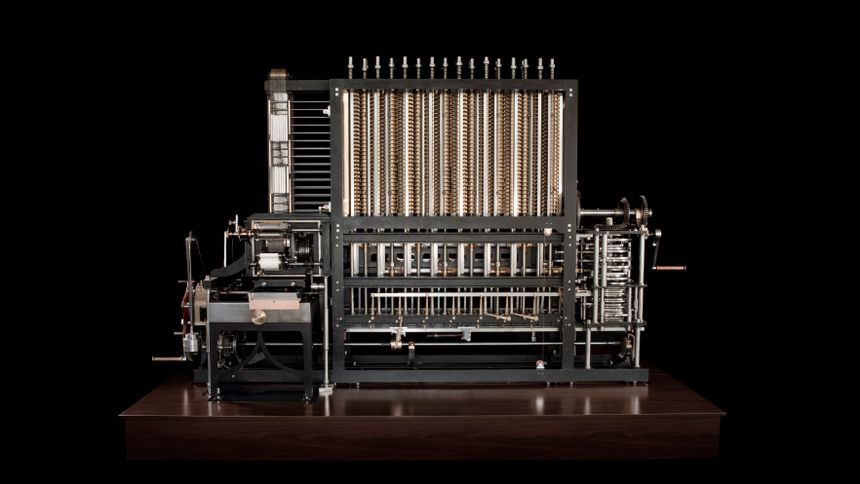
\includegraphics[scale=0.25]{pictures/bebidz.jpg}
\end{center}
\caption{Bebidžova diferencijska mašina}
\label{fig:beb}
\end{figure}

\subparagraph{Elektromehaničke mašine}
Ove mašine koristile su se od sredine $19.$ veka do Drugog svetskog rata.
Jednu od prvih mašina za čitanje bušenih kartica konstruisana je od strane Hermana Holerita. Njena glavna svrha bila je obrada rezultata popisa stanovništva u Sjedinjenim američkim državama 1890. godine. 
Koristeći bušene kartice uspešno izvršen je popis za godinu dana, naspram deset godina, koliko je bilo potrebno ranije. Od Holeritove male kompanije nastao je IBM.\footnote{Herman Hollerith (1860–1929), američki pronalazač.}

\subparagraph{Elektronski računari} Elektronski računari koriste se od kraja 1930-ih do
danas. 
 
\subsection{Fon Nojmanova arhitektura}
\label{sec:fN}
Na osnovu istorijata može se uočiti da svi navedeni računari imaju nedostatak jedne važne karakteristike računara danas, a to je programabilnost. Mašine korišćene nekada nisu bile programabilne već su funkcionisale po unapred definisanom programu određenom samom konstrukcijom mašine. Iako ovakav pristup nije sasvim izumro (danas se može videti na primeru digitrona), uglavnom nije poželjan. Prava promena u pristupu, koja je dovela do stvaranja programabilnih računara, nastala je ranih 1940-ih godina sa pojavom računara koji bi programe koje izvršavaju čuvali u memoriji zajedno sa podacima. Takve računare nazivamo računarima sa skladištenim podacima (engl. stored program computers). Jedna od najvažnijih karakteristika ovih računara je da kod njih postoji jasna podela na hardver i softver. Za rodonačelnika ovakve arhitekture smatra se Džon fon Nojman. On je 1945. godine opisao arhitekturu čija je glavna karakteristika da se programi mogu učitavati isto kao i podaci koji se obrađuju. Primeri prvih ovakvih računara su EDVAC, Mark 1 i EDSAC.\\\\
Osnovni elementi fon Nojmanove arhitekture su:
\begin{enumerate}
\item procesor - koji čine aritmetičko-logička jedinica, kontrolna jedinica i registri, i 
\item glavna memorija 
\end{enumerate}
koji su međusobno povezani, dok se ostale komponente računara smatraju pomoćnim. Prikaz fon Nojmanove arhitekture je na slici \ref{fig:fonN}.
\begin{figure}[h!]
\begin{center}
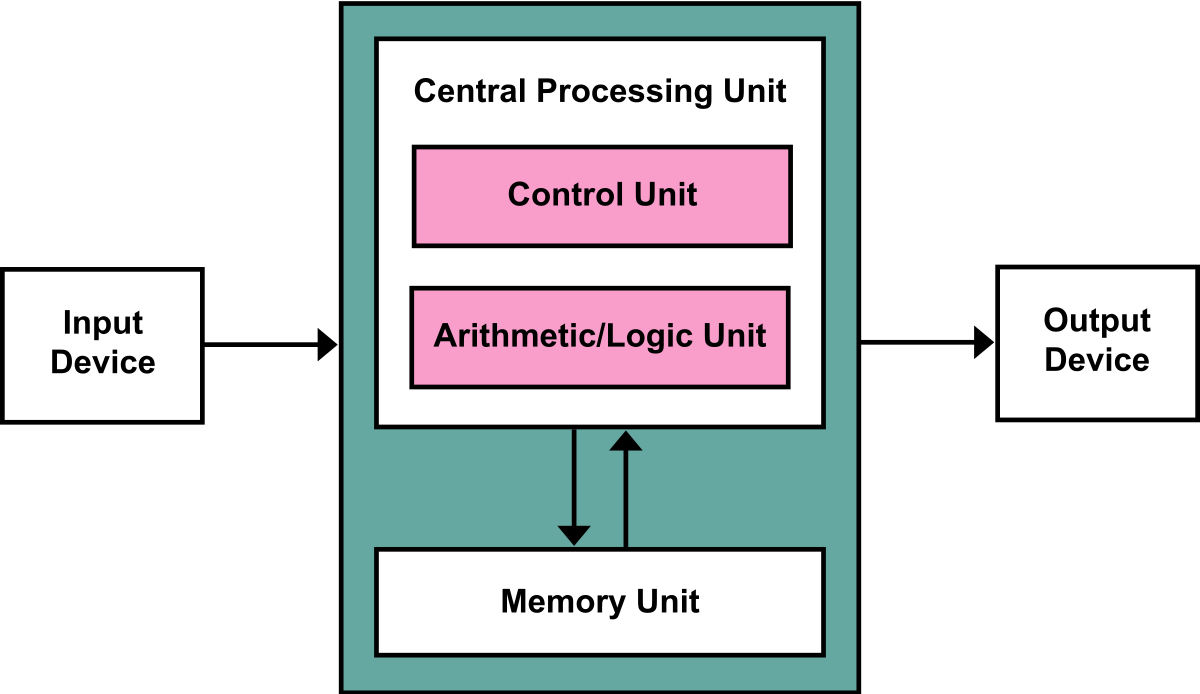
\includegraphics[scale=0.25]{pictures/fonN.png}
\end{center}
\caption{Šematski prikaz fon Nojmanove arhitekture}
\label{fig:fonN}
\end{figure}
Pod pomoćne komponente ubrajamo ulazno-izlazne jediice, spoljašnje memorije itd., koje da bi funkcionisale moraju biti povezane na centralni deo računara (procesor i glavnu memoriju).
Osnovna uloga procesora je obrada podataka, dok je osnovna uloga memorije skladištenje podataka koji se obrađuju, kao i programa. Postoji jedinstven način na koji zapisujemo i podatke i programe, a to je uz pomoć nula i jedinica, odnosno, binarnim zapisom. Tokom rada računara podaci i programi se prenose između procesora i glavne memorije.
\subparagraph{Procesor} Prva centralna komponenta fon Nojmanove arhitekture. Procesor, koji je odgovoran za rad računara, sastoji se od \textit{kontrolne jedinice} - koja upravlja radom procesora i \textit{aritmetičko-logičke jedinice} - koja je zadužena za izvođenje aritmetičkih operacija (sabiranje, oduzimanje, množenje, poređenje, itd. ) i logičkih operacija (konjunkcija, negacija, itd. ) nad brojevima. Osim dva navedena dela procesor sadrži i određeni broj registara, obično fiksirane širine (8, 16, 32 ili 64 bita), koji privremeno mogu da čuvaju podatke. Danas procesori neretko poseduju više jezgara (engl. core) koja istovremeno izvršavaju instrukcije čime se obezbeđuje paralelno izvršavanje.
\subparagraph{Memorija} Druga centralna komponenta fon Nojmanove arhitekture
je glavna memorija. Memorija predstavlja linearno uređeni niz registara, pri čemu svaki ima svoju adresu. Kao posledica osobine ove memorije da se sadržaju može pristupati u slučajnom redosledu, čest naziv je i memorija sa slobodnim pristupom (engl. RAM - random access memory). Razlikujemo nekoliko parametara koji odlikuju memoriju, to su:
\begin{itemize}
\item kapacitet - GB,
\item vreme pristupa - vreme potrebno da se memorija pripremi za čitanje ili upis i 
\item protok - izražava količinu podataka koji se prenose po jedinici merenja (danas obično mereno u GBps).
\end{itemize}
Na slici \ref{fig:memh} može se videti memorijska hijerarhija.
\begin{figure}[h!]
\begin{center}
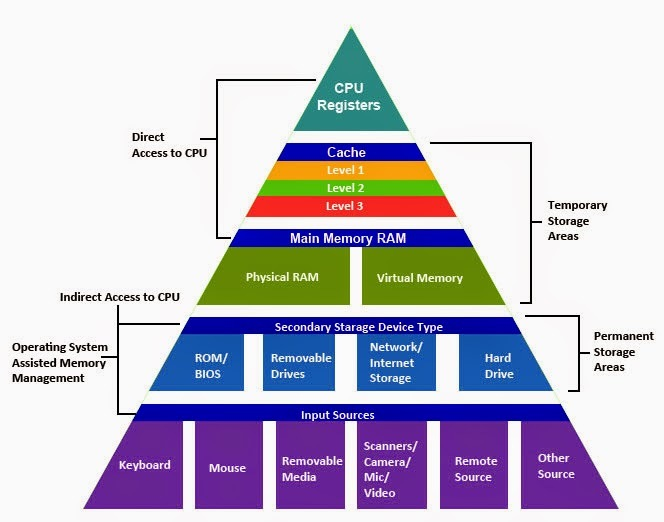
\includegraphics[scale=0.5]{pictures/mem_hijer.jpg}
\end{center}
\caption{Šematski prikaz memorijske hijerarhije}
\label{fig:memh}
\end{figure}

\subsection{Hardver}
Bez obzira na činjenicu da osnovu savremenih računarskih sistema i dalje čini fon Nojmanova arhitektura, za rad računara u današnjem smislu reči potreban je i čitav niz hardverskih komponenti koje nam dodatno olakšavaju. Opis komponenti koje čine jedan računar danas ne sastoji se od kućišta, monitora, tastature i miša, već nam je potreban apstraktniji, sveobuhvatniji opis. Upravo, kako bi se jasnije i preciznije opisao računar kaže se da ga čine:
\begin{itemize}
\item procesor tj. centralna procesorska jedinica (engl. Central Processing Unit,
CPU), koja obrađuje podatke,
\item glavna memorija (engl. main memory), u kojoj se istovremeno čuvaju i
podaci koji se obrađuju i trenutno pokrenuti programi, i 
\item različiti periferijski uređaji ili ulazno-izlazne jedinice (engl. peripherals,
input-output devices, IO devices), u koje se ubrajaju miševi, tastature, ekrani,
štampači, diskovi, a koji služe za interakciju između korisnika i sistema i trajno skladištenje podataka i programa.
\end{itemize} 
Da bi se izvršilo povezivanje svih navedenih komponenti koristimo magistralu.
Za funkcionisanje modernih računara neophodni su i hardver i softver. 
Hardver (tehnički sistem računara) čine opipljive, fizičke komponente računara: procesor, memorija, matična ploča, itd. 

\subsection{Softver}
Softver računara čine programi i prateći podaci koji određuju izračunavanja koja vrši računar.
Prvi računari su se odlikovali jezicima specifičnim za konkretni računar - mašinski zavisnim jezicima. Već od 1950-ih, sa pojavom prvih jezika višeg nivoa, programiranje postaje dosta lakše. Danas, programi se najčešće pišu u višim programskim jezicima, a potom se prevode na mašinski jezik, onaj koji je razumljiv računaru. Programom opisujemo računaru koje operacije treba da izvrši sa ciljem ispunjavanja nekog zadatka. U nastavku biće navedeno nekoliko primera koji ilustruju izvršavanje programa napisanih na višim programskim jezicima. 
\begin{primer}
Želimo da izračunamo vrednost izraza $2*x + 3$ za neko $x$. Podatke u računarstvu, kao i u matematici, možemo predstaviti pomoću promenljivih. Međutim, za razliku od matematike, promenljive u računarstvu mogu menjati svoju vrednost. Svakoj promenljivoj je u memoriji računara pridruženo jedno fiksirano mesto i ona može tokom izvršavanja programa da menja vrednost. Recimo da je $x$ ulazni parametar našeg programa, a $y$ izlazna vrednost, tada izračunavanje opisujemo sa
\begin{verbatim}
y := 2*x + 3
\end{verbatim}
gde $*$ označava množenje, $+$ sabiranje, a $:=$ naredbu dodele, odnosno promenljivoj sa leve strane izraza dodeljujemo vrednost izraza sa desne strane.
\end{primer}
\begin{primer}
Kao naredni primer uzmimo poređenje dva broja, odnosno, kao izlaz treba da dobijemo veći od dva broja.
Ovakav izraz možemo zapisati kao:
\begin{verbatim}
ako je x >= y onda
    m := x
inače
    m := y
\end{verbatim}
\end{primer}
\begin{primer}
Kao još jedan primer uzmimo stepenovanje:
\begin{verbatim}
s := 1, i := 0
dok je i < n radi sledeće:
    s := s·x, 
    i := i + 1
\end{verbatim}
\end{primer}
Savremeni softver klasifikujemo u 2 kategorije:
\begin{itemize}
\item Sistemski i
\item Aplikativni.
\end{itemize}
\textbf{\em Aplikativni softver} je onaj koji krajnji korisnici računara direktno koriste u svojim svakodnevnim aktivnostima. Tu spadaju, na primer, pregledači Veba, e-mail klijenti, kancelarijski softver (programi za kucanje teksta, izradu prezentacija,...), video igre, softver za prikaz slika, itd.\\
\textbf{\em Sistemski softver} ima ulogu da kontroliše hardver i pruža usluge aplikativnom softveru. Najznačajniji skup sistemskog softvera je operativni sistem (OS), ali u sistemski softver ubrajamo i različite uslužne programe: editore teksta, alate za programiranje (prevodioci, dibageri, profajleri, integrisana okruženja) i slično. Uloga operativnog sistema je da programeru pruži skup funkcija koje programer može da koristi kako bi ispunio određeni cilj, sakrivajući konkretne hardverske detalje - ovaj skup funkcija naziva se programski interfejs za pisanje aplikacija (engl. API - Application Programming Interface).

\subsection{Oblasti savremenog računarstva}
Savremeno računarstvo sastoji se iz više podoblasti između kojih nema jasnih granica. Prema klasifikaciji američke asocijacije ACM - Association for Computing Machinery, razlikujemo naredne podoblasti~\cite{Janicic}:
\begin{itemize}
\item Algoritmika (procesi izračunavanja i njihova složenost)
\item Strukture podataka (reprezentovanje i obrada podataka)
\item Programski jezici (dizajn i analiza svojstava formalnih jezika za opisivanje
algoritama)
\item Programiranje (proces zapisivanja algoritama u nekom programskom jeziku)
\item Softversko inženjerstvo (proces dizajniranja, razvoja i testiranja programa)
\item Prevođenje programskih jezika (efikasno prevođenje viših programskih jezika,
obično na mašinski jezik)
\item Operativni sistemi (sistemi za upravljanje računarom i programima)
\item Mrežno računarstvo (algoritmi i protokoli za komunikaciju između računara)
\item Primene (dizajn i razvoj softvera za svakodnevnu upotrebu)
\item Istraživanje podataka (pronalaženje relevantnih informacija u velikim skupovima
podataka)
\item Veštačka inteligencija (rešavanje problema u kojima se javlja kombinatorna
eksplozija)
\item Robotika (algoritmi za kontrolu ponašanja robota)
\item Računarska grafika (analiza i sinteza slika i animacija)
\item Kriptografija (algoritmi za zaštitu privatnosti podataka)
\item Teorijsko računarstvo (teorijske osnove izračunavanja, računarska matematika,
verifikacija softvera, itd).
\end{itemize}

\subsection{Osnovni pojmovi i konstrukti}
Programiranje predstavlja proces zapisivanja algoritama u nekom programskom jeziku.
Algoritam predstavlja precizan opis postupka za rešavanje nekog problema u konačnom broju koraka. Algoritmi se odlikuju svojom složenošću. Ta složenost može biti vremenska ili memorijska. Vremenska složenost se odnosi na vreme potrebno za izvršavanje nekog algoritma. Memorijska složenost označava koliko memorijskih resursa je potrebno za izvršavanje algoritma. Cilj analize algoritama je predviđanje njegovog ponašanja i brzine izvršavanja bez realizacije na nekom konkretnom računaru. Ta procena treba da se odnosi na svaki računar. Nemoguće bi bilo na svakom računaru ispitati izvršavanje nekog algoritma. Zbog toga je analiza algoritama približna tehnika.~\cite{Zivkovic} Postoji uniformna tehnika za grafički prikaz algoritama, međutim, mi nećemo ulaziti u detalje, već će biti dato nekoliko ilustrativnih primera kako bi se dobila glavna ideja.
\begin{primer}
Kao najjednostavniji primer algoritma uzmimo primer sa lampom. U početnom koraku lampa je ugašena, a mi želimo da je upalimo ili, ako ne radi, da je odnesemo na popravku. Najpre, proveravamo da li je lampa uključena u struju. Romb je znak kojim označavamo uslov. Ako lampa nije uključena u struju treba je uključiti. U suprotnom, ako je lampa uključena u struju, ali ne svetli, proveravamo da li je sijalica pregorela. Ako jeste, menjamo sijalicu. Ako nije, lampa je pokvarena i moramo je popraviti. Na slici \ref{fig:alg0} vidimo kako bismo grafički prikazali opisani postupak.
\begin{figure}[h!]
\begin{center}
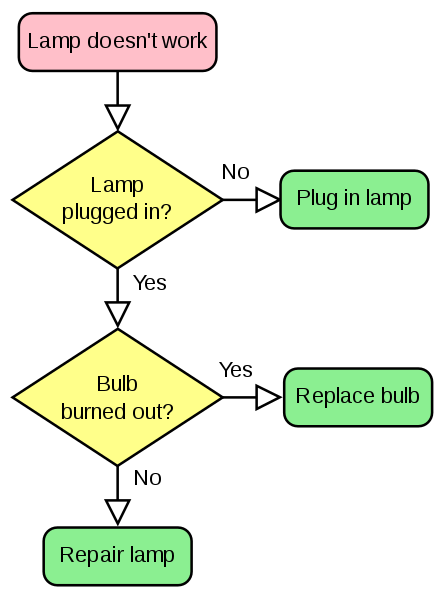
\includegraphics[scale=0.25]{pictures/lamp.png}
\end{center}
\caption{Primer najjednostavnijeg algoritma.}
\label{fig:alg0}
\end{figure}
\end{primer}

\begin{primer}
Kao primer, više prikladan računarskoj terminologiji, uzmimo sabiranje $2$ broja, $M$ i $N$. Na slici \ref{fig:alg1} vidimo kako bismo grafički prikazali postupak sabiranja brojeva.
\begin{figure}[h!]
\begin{center}
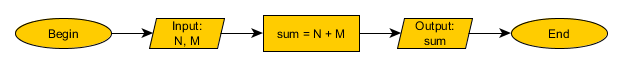
\includegraphics[scale=0.5]{pictures/sum-num-alg.png}
\end{center}
\caption{Prikaz algoritma za sabiranje dva broja.}
\label{fig:alg1}
\end{figure}
\end{primer}

U sekciji \ref{sec:fN} koja govori o fon Nojmanovoj arhitekturi, videli smo da se podaci (i programi) smeštaju u memoriju računara, najčešće u vidu niza bitova. Međutim, kako se programer ne bi zamarao detaljima i kako bi mogao da radi na dosta apstraktnijem nivou, programski jezici obezbeđuju koncept promenljivih. Promenljive daju mogućnost programeru da podacima dodeli imena i da im na osnovu tih imena i pristupa. Svaka promenljiva u programu ima dodeljen određeni niz bajtova. \\\\
Promenenljive se odlikuju svojim tipovima i životnim vekom. Životni vek je koncept koji nam govori u kom delu faze izvršavanja programa je promenljivoj dodeljen memorijski prostor, odnosno, kada je možemo koristiti. Životni vek promenljive omogućava da na različitim mestima u programu koristimo različite promenljive istog imena i pravilo dosega identifikatora (engl. scope) određuje deo programa u kome se uvedeno ime može koristiti. Druga odlika promenljivih su tipovi. Organizovanje podataka u tipove pomaže programeru da ne mora da razmišlja o podacima na nivou njihove binarne reprezentacije, već daleko apstraktnije. Neki od najčešćih tipova su:
\begin{itemize}
\item celi brojevi (... -3, -2, -1, 0, 1, 2, 3,...),
\item brojevi u pokretnom zarezu ( 1.0, 3.14, 9.81,...),
\item karakteri (a, b, P, ,, !, ...),
\item niske ("zdravo", "svima",...)
\end{itemize} 
Osim ovih postoje i složeniji tipovi koji mogu objediniti više istih ili različitih tipova, pa tako imamo nizove, strukture, liste, i dr.
Svaki tip podataka se karakteriše vrstom podataka koje opisuje, skupom operacija koje se nad njime vrše i načinom reprezentacije i detaljima implementacije tog tipa.

Osnovni gradivni elementi imperativnih programskih jezika su naredbe.
Naredba dodele je osnovna naredba i njom se vrednost neke promenljive postavlja na vrednost nekog izraza definisanog nad konstantama i promenljivim. Šta to, u praksi, znači? To znači da kada kažemo $x = 3*y$ zapravo promenljivoj x dodeljujemo vrednost $3*y$. Naredbe se u programu nižu jedna za drugom, osim u slučaju korišćenja naredbi za kontrolu toka izvršavanja programa. Ove naredbe u zavisnosti od tekućih
vrednosti promenljivih neke naredbe mogu da ne izvršavaju, izvršavaju ih više puta(petlje) i slično. Najčešće korišćene kontrolne strukture su granajuće naredbe (if-then-else), petlje (for, while, do-while, repeat-until) i naredbe skoka (goto). Naredba if-then-else ima sledeći opšti oblik:
\begin{verbatim}
if izraz1 
   naredba1
else 
   naredba2
\end{verbatim}
Treba obratiti pažnju da je else grana neobavezna, odnosno, može, ali ne mora, da postoji. 
\begin{primer}
Naredni primer štampa veći od dva broja.
\begin{verbatim}
if a > b
   print(a)
else
   print(b)
\end{verbatim}
\end{primer}

\begin{primer}
Naredni primer u promenljivu $a$ smešta tekst $"$Hello world!$"$ ako je vrednost promenljive b veća od 0.
\begin{verbatim}
if b > 0
   a = "Hello world!"
\end{verbatim}
\end{primer}

Jedan od najbitnijih koncepata programiranja je pojam {\em petlje}. Petlje predstavljaju konstrukcije koje nam omogućuju da izvršavamo jednu ili više akcija više puta. Sastoje se iz uslova i tela petlje. Uslov nam definiše u kom slučaju ćemo napustiti petlju (na primer, ako broj iteracija\footnote{Iteracija petlje predstavlja jedno izvršavanje koda koji se nalazi u telu petlje.} petlje predje 100, ili ako je neka promenljiva n veca od 1000, itd.). Telo petlje sadrži akcije koje želimo da ponavljamo.Na slici \ref{fig:loops} može se videti opšti oblik petlji.
\begin{figure}[h!]
\begin{center}
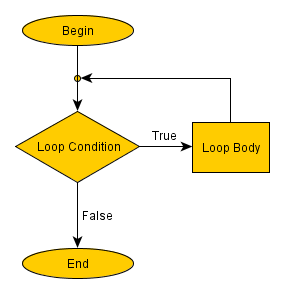
\includegraphics[scale=0.5]{pictures/Loops.png}
\end{center}
\caption{Petlja.}
\label{fig:loops}
\end{figure}

\begin{primer}
Za naredni primer, uzećemo sabiranje prvih 50 brojeva. Naime, naporno bi bilo da pišemo $1+2+3+...+50$, a da ne pomišljamo na brojeve poput $1000$, $100 000$ ili $1 000 000$. To bi bilo gotovo neizvodivo. Zbog toga, želimo da na apstraktniji način opišemo proceduru koja će umesto nas izvršiti sabiranje prvih 50 brojeva. Da bismo to uspeli moramo iskoristiti petlju. Na slici \ref{fig:alg2} vidimo kako bismo grafički prikazali postupak.
\begin{figure}[h!]
\begin{center}
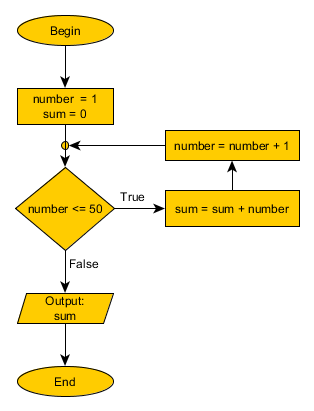
\includegraphics[scale=0.5]{pictures/algorithm-flow.png}
\end{center}
\caption{Prikaz algoritma za sabiranje prvih 50 brojeva.}
\label{fig:alg2}
\end{figure}
\end{primer}

Petlje su neophodne za uspešno programiranje. 
 Postoji nekoliko različitih vrsta petlji,  čija upotreba zavisi od onoga što njom želimo da postignemo, pa tako imamo:
\begin{itemize}
\item $"for"$ petlju i
\item $"while"$ petlju 
\end{itemize}
koje predstavljaju osnovne konstrukte u skoro svim programskim jezicima. Osim for i while petlje postoje i druge, ali o njima nece biti reči.\\\\
For petlja je najčešće oblika:
\begin{verbatim}
for(izraz1, izraz2, izraz3)
    naredba
\end{verbatim}
$Izraz1$ i $izraz3$ obično predstavljaju naredbe dodele ili inkrementiranje, gde se $izraz1$ obično naziva inicijalizacija, a $izraz3$ je korak. Izraz u sredini, $izraz2$, predstavlja relacijski izraz i služi kao uslov izlaska iz petlje. $Naredba$ predstavlja liniju ili blok koda koji želimo da se izvršava.
Kao posledica navedenog, $for$ petlju možemo posmatrati kao:
\begin{verbatim}
for(inicijalizacija, uslov izlaska, korak)
    kod koji želimo da se izvrši
\end{verbatim}
\begin{primer}
Naredni primer predstavlja jedan od uobičajenih oblika u kojima se $for$ petlja pojavljuje:
\begin{verbatim}
for(i = 0; i < n; i++)
    print(i)
\end{verbatim}
Ovaj primer za svaki korak petlje ispisuje broj koraka. 
\end{primer}


\subsection{Klasifikacija programskih jezika}

Brojnost programskih jezika raste iz godine u godinu. Stalno se pojavljuju novi i brži jezici, unapređuju se stari i nemoguće je ispratiti sve promene. Da bismo odmah razumeli okvirno kako neki programski jezik funkcioniše moramo znati kojoj paradigmi pripada. Kada kažemo da neki jezik pripada nekoj paradigmi mi zapravo govorimo nešto o karakteristikama tog jezika koje važe za sve jezike koji pripadaju istoj grupi. Programske paradigme su formirane prema načinu programiranja. Neki od najkorišćenijih programskih jezika današnjice spadaju u grupu imperativnih programskih jezika, npr. jezik C. Glavna karakteristika imperativnih programskih jezika je da stanje programa karakterišu promenljive kojima se predstavljaju podaci i naredbe kojima se vrše određene transformacije nad promenljivim (sabiranje, oduzimanje, poređenje, itd.). Osim imperativne, značajne programske paradigme su i
objektno-orijentisana (C++, Java (Java NIJE JavaScript!), C\# itd.), funkcionalna (Lisp, Haskell, ML, itd.), logička (u nju spada, na primer, Prolog). Sa razvojem savremenih programskih jezika došlo je do brisanja jasnih granica između ovih jezika, pa tako dolazi do mešanja karakteristika različitih paradigmi.\\\\
Za većinu programskih jezika danas reći ćemo da su proceduralni. Kada kažemo da je neki jezik proceduralan zapravo želimo da iskažemo činjenicu da je zadatak programera da opiše način (proceduru) kojim će se doći do rešenja problema. Kao idejno potpuno kontrastni, postoje deklarativni programski jezici (poput Prologa) koji od programera zahteva precizan opis problema, a mehanizam programskog jezika se onda bavi pronalaskom rešenja.\\\\
Prema tipu konverzije tipova imamo statički i dinamički tipizirane jezike. Kod statički tipiziranih jezika (poput C-a) zahteva se da programer definiše tip svake promenljive i da ga potom više ne menja tokom izvršavanja programa. Kod dinamički tipiziranih jezika ista promenljiva može sadržati podatke različitog tipa tokom različitih faza izvršavanja. Nekada je moguće čak i vršenje operacija nad promenljivima različitog tipa, pri čemu dolazi do implicitne konverzije. Na primer, jezik JavaScript ne zahteva definisanje tipa promenjlivih i dopušta kôd poput $a = 1; b = "2"; a = a + b;$\\\\

\subsection{Primeri za vežbu}
\begin{primer}
Napisati primer algoritma za kuvanje kafe.
\end{primer}
\begin{primer}
Napisati primer algoritma za provodjenje jednog dana.
\end{primer}
\begin{primer}
Napisati primer algoritma za savladavanje nekog kursa. 
\end{primer}
\begin{primer}
Napisati primer algoritma za računanje zbira prvih 10 parnih brojeva.
\end{primer}
\begin{primer}
Koju vrednost ima promenljiva $x$ nakon izvršavanja narednog koda:
\begin{verbatim}
int x = 0;
if (x > 3);
    x++;
\end{verbatim}
\end{primer}
\begin{primer}
Napisati pseudo kod za računanje zbira 3 broja.
\end{primer}
\begin{primer}
Napisati pseudo kod u kome se promenljivoj $a$ dodeljuje vrednost $3$, promenljivoj $b$ dodeljuje vrednost $6$ i onda se njihov zbir smešta u promenljivu $c$. Nakon toga, proveriti da li ostatak pri deljenju promenljive (računa se uz pomoć \%) $c$ sa brojem 2 daje 0, odnosno, da li je $c$ paran.
\end{primer}
\begin{primer}
Napisati pseudo kod\footnote{Pseudo kod predstavlja kod koji nije dat u formalnim terminima, već predstavlja ideju kako bi kod trebao da izgleda.} algoritma za računanje zbira prvih 10 parnih brojeva.
\end{primer}
\begin{primer}

\end{primer}

\subsection{Domaći zadatak}
Domaći zadatak:
\begin{itemize}
\item pročitati nešto dodatno o istorijatu računarstva (01\_istorijat), 
\item opisati ukratko svaki od elemenata memorije (01\_piramida),
\item odraditi sve primere i pitalice ,
\item domaci sa osi/tcp slojevima: 01\_osi, 01\_tcp
\item domaci koji je size teksta o browserima: 01\_browser
\item samostalno pronaći još 10 novih i uraditi ih(01\_0,...,01\_9).
\end{itemize}
\newpage
\section{Uvod u web}
\label{sec:uvodweb}
Danas, ne možemo zamisliti korišćenje računara bez veza ka drugim računarima. Izgradnja računarskih mreža, a posebno sa nastankom i razvojem Interneta i njegovih servisa poput Veba, dovele su do porasta broja korisnika računara i promene uloga računara u odnosu na ranije. Pojava savremenih računarskih mreža smatra se revolucionarnom poput pojave parne mašine u $18.$ veku. Svake godine uvećava se broj umreženih računara, a sa tim brojem raste i broj usluga koje nam mrežno okruženje nudi. Neke od osnovnih primera upotreba računarskih mreža obuhvataju:
\begin{itemize}
\item poslovna: elektronska pošta, razmena datoteka, deljeni štampači, ...
\item kućna: filmovi, muzika, igrice, vesti, audio i video komunikacija, razmena poruka, elektronska kupovina,...
\item mobilne: pozivi, SMS, igrice, mape, pristup informacijama
\end{itemize}

\subsection{Uloga računarskih mreža}
U osnovne uloge računarskih mreža ubrajamo:
\begin{enumerate}

\item komunikaciju - uz pomoć računara ljudi razmenjuju poruke, video pozive, mejlove, ćaskanja (eng. chat), video konferencije, itd.
\item deljenje informacija i podataka - ako postoji mrežno okruženje u kom su računari povezani, tada je moguće pristupiti informacijama na drugim računarima u okviru mreže. Podatke prenosimo na više načina, kao što su preuzimanje datoteka, prenos informacija u okviru lokalnih mreža (obično u okviru jedne kompanije), kao i u okviru globalne svetske mreže. Internet i veb se smatraju glavnim izvorima informacija. 
\item deljenje softvera - korisnici povezani u mrežu mogu koristiti mnoge usluge koje im pruža softver koji radi na računarima u okviru mreže. Neke od usluga su kupovina i rezervacija karata preko interneta, ili izvršavanje softvera koji je distribuiran i paralelizovan na više povezanih računara, čime se može ubrzati izvršavanje.
\item deljenje hardverskih resursa - obezbeđuje zajedničko korišćenje hardvera, poput štampača, skenera i ostalih. Često se ovakav pristup koristi u kompanijama.
\end{enumerate} 

Računarski resursi u mreži mogu biti raspoređeni na različite načine, tako da obezbeđuju različite načine izvršavanja poslova. Neki od najčešćih su:
\begin{itemize}
\item Centralizovana obrada - svi poslovi se izvršavaju na jednom centralnom računaru, dok se ostali uređaji u mreži koriste samo kao terminali za unos podataka i prikaz rezultata. Ovakavim načinom rada odlikovale su se rane računarske mreže.
\item Klijent-server okruženje - jedan računar ima ulogu servera na kome se nalaze
podaci i aplikativni softver, koji se stavljaju na raspolaganje klijentima. Serveri su obično moćniji računari od klijenata(mada ne mora uvek biti tako) i na njima se obavljaju zadaci koji zahtevaju više resursa. U današnjem kontekstu, stroga podela na klijentski i serverski računar više nije tako aktuelna. Najčešće govorimo o tome da je jedan računar istovremeno i klijent i server u zavisnosti od zadataka koji su mu zadati. Na primer, isti računar može istovremeno pokretati i Veb server i klijent za elektronsku poštu, čime mu je data i uloga servera i uloga klijenta.
na njihov zahtev. 
\item Mreža ravnopravnih računara (eng. peer-to-peer - $P2P$) - računari direktno komuniciraju deleći podatke i opremu. Sve se češće ovakve mreže koriste za masovnu razmenu velikih količina podataka (npr. torenti - Bittorrent).
\end{itemize}
\begin{figure}[h!]
\begin{center}
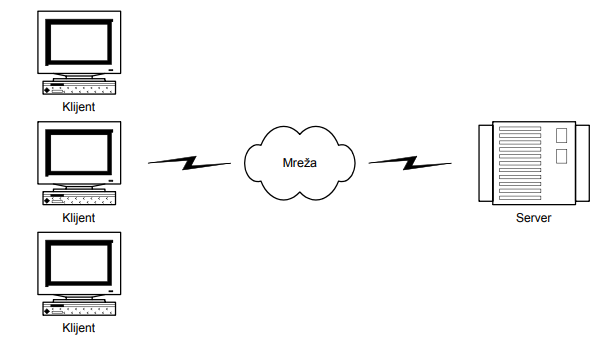
\includegraphics[scale=0.5]{pictures/KS.png}
\end{center}
\caption{Prikaz klijent-server arhitekture.}
\label{fig:KS}
\end{figure}

\subsection{Komponente računarskih mreža}
Pre nego što uđemo u detaljniji opis elemenata koji čine jednu računarsku mrežu, trebalo bi da damo formalnu definiciju šta je računarska mreža. Naime, računarska mreža je sistem koji se sastoji iz skupa hardverskih uređaja koji su međusobno povezani komunikacijskom opremom i koji je snabdeven odgovarajućim kontrolnim softverom kojim se ostvaruje kontrola funkcionisanja sistema tako da je moguć prenos podataka između povezanih uređaja. Neke od osnovnih komponenti računarskih mreža su, dakle:
\begin{itemize}
\item mrežni hardver, 
\item komunikacioni kanali i 
\item mrežni softver.
\end{itemize}

\begin{figure}[h!]
\begin{center}
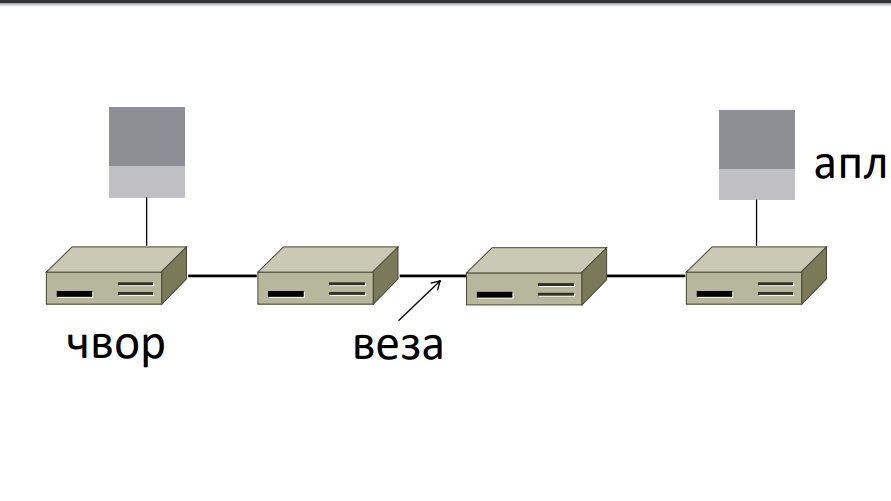
\includegraphics[scale=0.5]{pictures/PrMr.png}
\end{center}
\caption{Prikaz mreže.}
\label{fig:PrMr}
\end{figure}

\subsubsection{Mrežni hardver}
Tradicionalno, podrazumeva se povezivanje računara u okviru mreže, ili uz dodatak nekih pomoćnih uređaja poput štampača, skenera itd., kako bi se mogli deljeno koristiti. Međutim, u poslednje vreme, granica između klasičnih računara i digitalnih uređaja specijalizovane namene se briše i sve češće se u oviru mreže mogu povezati i PDA uređaji, mobilni telefoni, foto aparati, kamere i ostali. Aktivno se radi i na razvoju automobila, frižidera i ostalih mnogobrojnih uređaja kako bi se uključili u mrežu i kako bi se time omogućilo upravljanje istima na daljinu.\\\\
Da bismo neki uređaj mogli da ubacimo u mrežu, neophodno je da sadrži određene hardverske komponente koje bi mu to omogućile. Deo hardvera koji je namenjen za umrežavanje i spada u komunikacionu opremu je mrežna kartica ili mrežni adapter (eng. NIC - network interface card) koja omogućava fizički pristup mreži. Svaka mrežna kartica ima svoju jedinstvenu fizičku (MAC) adresu, kojom se uređaj jedinstveno identifikuje prilikom komunikacije. Neke mrežne kartice obezbeđuju pristup žičanim, a neke druge bežičnim komunikacionim kanalima. Osim mrežnih kartica za umrežavanje se koriste i modemi (telefonski, kablovski), kao i još neki uređaji o kojima neće biti reči. 
\begin{figure}[h!]
\begin{center}
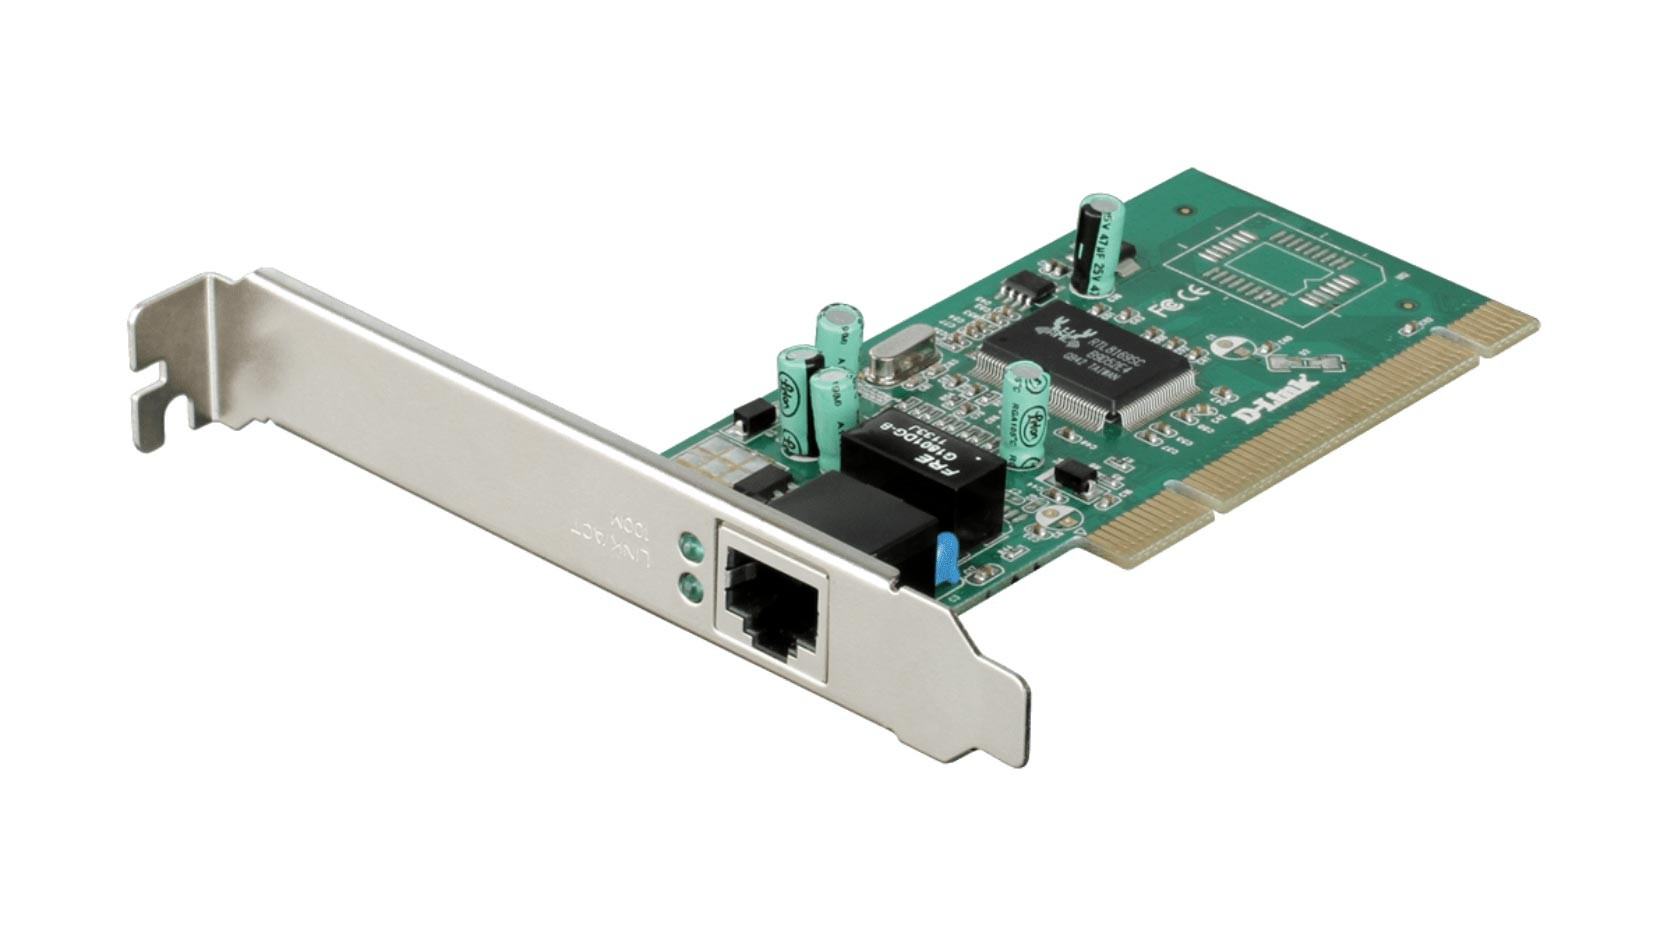
\includegraphics[scale=0.25]{pictures/mreznakartica.jpg}
\end{center}
\caption{Prikaz mrežne kartice.}
\label{fig:mk}
\end{figure}


\subsubsection{Komunikacioni kanali}
Da bi mreža funkcionisala i da bi kroz nju bilo moguće preneti podatke, uređaji koji se nalaze u mreži moraju biti povezani međusobno uz pomoć žičanih ili bežičnih prenosnih sistema, koji predstavljaju komunikacione kanale. Osnovna mera kvaliteta komunikacionog kanala je brzina prenosa koja se meri u bitovima po sekundi (bit/s). Ova mera označava broj bitova koji se mogu preneti kroz komunikacioni kanal u jednoj sekundi. Ako bismo posmatrali aktuelne tehnologije prenosa podataka, najčešće se koriste megabiti ( milion bita) u sekundi - Mbps, ili gigabiti (milijarda bita) u sekundi - Gbps. Brzina prenosa predstavlja fizičku karakteristiku komunikacionog kanala i zavisi od frekvencijskog opsega (eng. bandwidth) koji se može propustiti kroz kanala bez gubitka signala. Na slici \ref{fig:opseg} prikayan je raspon frekvencija za razne prenosne tehnologije. \\\\

\begin{figure}[h!]
\begin{center}
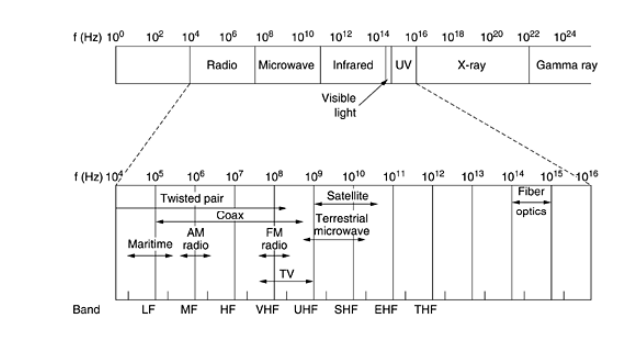
\includegraphics[scale=0.7]{pictures/bandw.png}
\end{center}
\caption{Prikaz frekvencijskih opsega za razne prenosne tehnologije.}
\label{fig:opseg}
\end{figure}

Komunikacione kanale možemo podeliti u dve grupe prema tipu prenosa informacija:
\begin{enumerate}
\item Žičane  
\item Bežične 
\end{enumerate}

\subparagraph{Žičane komunikacije} 
\subparagraph{Parice}(eng. twisted-pair wire) - Najkorišćeniji način komunikacije. Uređaji se povezuju korišćenjem uvijenih uparenih izolovanih bakarnih žica. Žice se uparuju i uvijaju kako bi se smanjile smetnje u komunikaciji. Brzina prenosa kroz ovakav medijum obično varira od $2Mbps$ do $100Mbps$.
\begin{figure}[h!]
\begin{center}
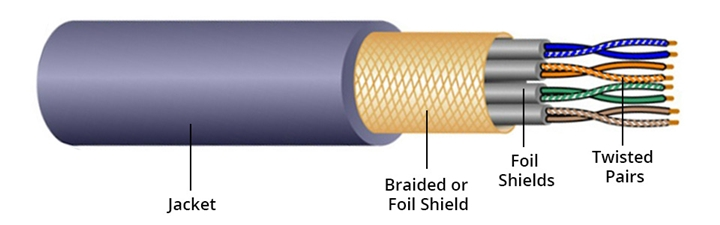
\includegraphics[scale=0.5]{pictures/twpw.jpg}
\end{center}
\caption{Prikaz parice.}
\label{fig:twpw}
\end{figure}

\subparagraph{Koaksijalni kablovi} svoju upotrebu najčešće nalaze u televizijskim kablovskim sistemima, a koriste se i u lokalnim mrežama u kompanijama. Kablovi se sastoje od centralne bakarne ili aluminijumske žice obmotane savitljivim slojem izolacije, oko kog je obmotan provodni sloj tankih žica, a potom je sve to izolovano. Ovaj tip kablova omogućava brzinu prenosa do $200Mbps$ (nekad čak i do $500Mbps$), uz manju osetljivost na elektromagnetne smetnje. 

\begin{figure}[h!]
\begin{center}
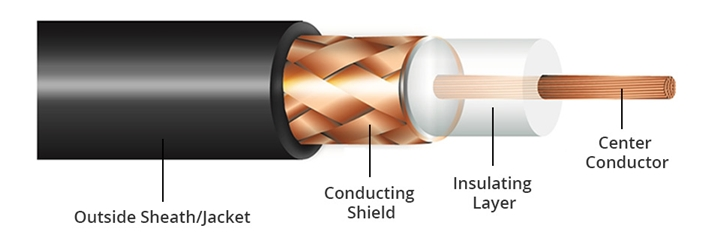
\includegraphics[scale=0.5]{pictures/coax.jpg}
\end{center}
\caption{Prikaz koaksijalnog kabla.}
\label{fig:coax}
\end{figure}

\subparagraph{Optički kablovi}- prave se od velikog broja (reda veličine nekoliko stotina ili hiljada) veoma tankih staklenih vlakana. Podaci se prenose svetlosnim talasima uz pomoć malog laserskog uređaja. Na ovaj tip kablova elektromagnetne smetnje nemaju uticaja. Najveći nedostatak ovakvih kablova je cena, izuzetno su skupi i komplikovani za komunikaciju, pa se uglavnom koriste za osovinski deo mreže, na koji se potom drugim vrstama kablova povezuju pojedinačni uređaji. Brzina ovih uređaja predstavlja njihovu najveću prednost. Naime, brzina ovih uređaja može ići i do nekoliko triliona bita u sekundi. Najčešće se koriste za mreže sa brzinama do $10 Gbps$.
\begin{figure}[h!]
\begin{center}
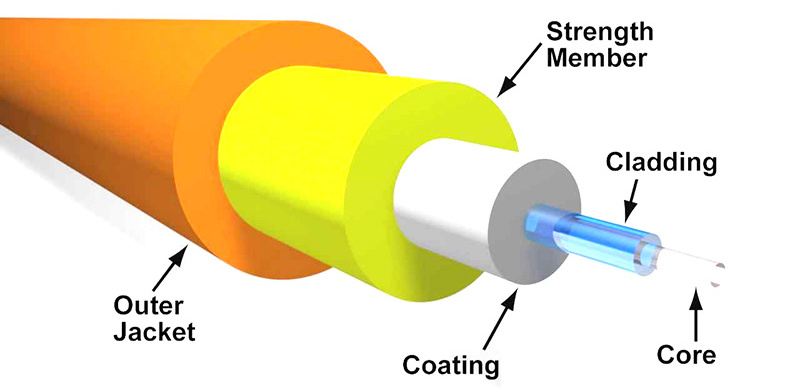
\includegraphics[scale=0.5]{pictures/optical.jpg}
\end{center}
\caption{Prikaz optičkog kabla.}
\label{fig:optical}
\end{figure}

\subparagraph{Bežične komunikacije}
Bežična komunikacija, kao što i samo ime sugeriše, ne koristi kablove za prenos podataka. Ovakav vid komunikacije poseban značaj nalazi kod prenosivih računara, mobilnih telefona ili dosta udaljenih lokacija do kojih bi bilo jako skupo, ako ne i nemoguće, sprovesti kablovsku mrežu. Umesto kablova ove mreže koriste radio talase, mikro talase i infracrvene zrake. Podaci se prenose moduliranjem amplitude, frekvencije ili faze talasa. Neke od danas najkorišćenijih tehnologija su: 
\begin{itemize}
\item Bluetooth - koristi se za veoma male razdaljine (do $10$ ili do $100$ metara. Brzina prenosa je do $3Mbps$. Bluetooth tehnologija koristi radio talase i može da prođe i kroz čvrste prepreke. Koristi se najčešće za komunikaciju računara sa periferjskim uređajima, kao i u mobilnoj telefoniji.
\item Bežični LAN - Wireless LAN (WLAN, WiFi) je tehnologija koja korsti radio talase za bežičnu komunikaciju više uređaja na ograničenim rastojanjima (nekoliko desetina ili stotina metara). Brzina prenosa ide od $10Mbps$ do $50Mbps$ ( u skorije vreme može ići i do $600Mbps$). Najrašireniji standard za ovaj vid komunikacije je IEEE $802.11$, o kome će kasnije biti više reči. 
\item Ćelijski sistemi - Način prenosa je sličan onom koji se koristi u mobilnoj telefoniji. Za komunikaciju se koriste radio talasi i sistemi antena koji pokrivaju određenu geografsku oblast, pri čemu se signal do cilja prenosi preko niza antena. 
\item Zemaljski mikrotalasi - koriste antensku mrežu na Zemlji, a za komunikaciju koriste mikrotalase niske frekvencije koji zahtevaju da antene budu optički vidljive, pa se iste smeštaju na visoke tačke. 
\item Komunikacioni sateliti - koriste mikrotalase za komunikaciju tako što se prenos između dve tačke koje nemaju optičku vidljivost ostvaruje poprečnom komunikacijom preko satelita koji se nalaze u orbiti. Na ovaj način se prenose televizijski i telefonijski signal. Brzina komunikacije je dosta mala $100Mbps$.
\end{itemize}

\subsubsection{Mrežni softver}
Mrežna infrastruktura sama po sebi ne služi ničemu bez mrežnog softvera. Uloga mrežnog softvera je da obezbedi korisniku mrežnu komunikaciju. Na primer, programer pregledača Veba, ne treba da misli o tome kako će pregledač primiti informacije, već treba da se fokusira samo na aspekte značajne za njegovu konkretnu aplikaciju, a sve ostale detalje prepusti nižem sloju mrežnog softvera.

Mrežni softver, najgrublje, može da se podeli na dva nivoa:
\begin{itemize}
\item niskog nivoa - mrežni softver koji omogućuje korišćenje različitih mrežnih uređaja, poput mrežnih kartica, modema, itd. Ovaj softver se nalazi u jezgru operativnog sistema i u obliku upravljača perifernim uređajima, takoznavnih drajvera (eng. driver). On upravlja računarskim hardverom i komunikacijskom opremom. Korisnik nikad ne koristi ovaj softver direktno, a često nije ni svestan njegovog postojanja 
\item visokog nivoa.
\end{itemize}

\subsection{Literatura}
Čitanje literature predstavlja neizostavan deo gradiva, kako naredni izvori predstavljaju odlican izvor informacija, na vama je da ih procitate:
\begin{itemize}
\item Predrag Janičić, Programiranje 1, Matematički fakultet, glava 1
\item Filip Marić, Uvod u web i internet tehnologije, Matematički fakultet, glave 1 i 2
\item Ajzenhamer Nikola, Bukurov Anja, Stanković Vojislav, Programiranje za Veb skripta, glave 1,2 i 3
\end{itemize}
\newpage

\section{HTML i CSS}
\label{sec:htmlcss}
HTML i CSS predstavljanju neizostavan materijal pri učenju web programiranja. Upravo zbog njihovog velikog značaja im posvećujem celo poglavlje. Slajdovi korišćeni prilikom predavanja su apsolutno nedovoljan materijal. Svi materijali korišćeni pri kreiranju časova, kao i ovog materijala su javno dostupni i nalaze se na:
\begin{itemize}
\item Aleksandar Veljković, Veb programiranje, Matematički fakultet http://poincare.matf.bg.ac.rs/~aleksandar/files/web/skripta.pdf
\item W3Schools: https://www.w3schools.com/
\item Filip Marić, Uvod u Veb i Internet tehnologije, Matematički fakultet 
\end{itemize}

\subsection{HTML}
\subsubsection{Zadaci sa časa}
Neki od zadataka rađenih na času su navedeni u nastavku.

\begin{primer}
Prva HTML stranica: Treba kreirati svoju prvu HTML stranicu korišćenjem tagova. Propozicije stranice su sledeće:
\begin{itemize}
\item Kreirati naslov stranice i iskoristiti barem 3 nivoa heading-a
\item Napisati neki pasus koji ima smisla, u okviru kog treba iskoristiti break, strong i em tagove
\item Potom kreirati isto to za ostale nivoe headinga
\item Kreirati jos barem 3 stranice, od čega: 2 treba da sadrže smisleni tekst u paragrafima, a poslednja može sadržati tekst u vidu \textit{lorem ipsum dolor sit...}
\item Druga strana treba da sadrži linkove ka barem 3 spoljašnje strane, npr: ujutru uz kafu volim da čitam, pa linkove ka nekoliko portala
\item Svaka strana treba da sadrži veze ka svim ostalim stranama
\end{itemize}
\end{primer}

\begin{primer}
Španska kuhinja: Kreirati sajt prema sledećim propozicijama:
\begin{enumerate}
\item Iz kojih jela se sastoje tipični obroci u Španiji (entrada, primer plato, segundo plato,...)?
\item Kreirati osnovnu stranicu sa opisom delova obroka, a potom za svaki deo obroka kreirati posebnu stranicu.
\item Svaka stranica mora da sadrži
	\begin{itemize}
		\item Naslov, npr.: Primer plato
		\item Podnaslov, naziv nekog tipičnog jela karakterističnog za taj obrok, npr.: Nachos (za entradas)
		\item Pasus, nešto o tom jelu, odakle je poteklo, kad je nastalo  i slično
		\item Pasus sa neuređenom listom potrebnih sastojaka
		\item Pasus sa uređenom listom postupka pripreme
	\end{itemize}
\item Nekoliko slika jela
\item Vezu ka prethodnoj i narednoj stranici
\item Poslednja stranica treba da se vraća na prvu i da ima spoljašnju vezu ka opisu nekog grada u Španiji.
\end{enumerate}
\end{primer}
\begin{primer}
Sportski izveštaj: Kreirati stranicu o sportu. Odabrati sport po izboru, a potom ispuniti specifikaciju:
\begin{enumerate}
\item Napraviti definicionu listu koja opisuje odabrani sport
\item Napraviti listu sa pravilima igre, ako je moguće kreirati listu u listi (ugnježdena lista)
\item Kreirati tabelu sa rezultatima nekog takmičenja
\item Ubaciti dve ili više slika (iskoristiti width i height kako bi se veličina slike prilagodila)
\item Ubaciti tabelu sa rezultatima sa nekog većeg takmičenja iz tog sporta
\end{enumerate}
\end{primer}
\begin{primer}
Stiven Hoking: Kreirati sajt koji će sadržati informacije o Stivenu Hokingu (eng. Stephen Hawking).
Specifikacija sajta je sledeća:
\begin{itemize}
\item Sajt treba da sadrži naslov, kome će u tooltip-u stajati: engleski teoretski fizičar, kosmolog, autor i direktor istaživanja u Centru za teorijsku kosmologiju na Univerzitetu u Kembrdžu.
\item Ispod naslova treba da stoji kratki paragraf o Stivenu Hokingu, paragraf treba da sadrži boldovan i italic tekst, kao i nešto što bi bilo highlightovano i precrtano
\item Kreirati listu sa spiskom njegovih publikacija
\item Ubaciti sliku, i skalirati je korišćenjem odgovarajućih atributa
\item Ubaciti neki citat na odgovarajući način
\item Ubaciti citat nečega sa njegove stranice, i potom referisati stranicu.
\item Ubaciti vezu ka drugoj stranici na kojoj će biti slike i nazivi nekih od njegovih publikacija
\end{itemize}
\end{primer}

\begin{primer}
Forma za registraciju za učešće na nekom kursu. Zadatak je kreirati stranicu koja će sadržati formu, koja bi trebalo da se popuni kako bi se prijavilo za učešće na nekom od kurseva. Sami odaberite nazive kurseva, kao i relevantne informacije polaznika.
\begin{itemize}
\item Ime
\item Prezime
\item Adresa
\item Grad
\item Broj telefona
\item Broj mobilnog
\item e-mail adresa
\item kurs za koji se prijavljuje - lista od barem 5 izbora
\item odabir termina: vikendom, radnim danima ili svejedno - radio buttoni
\item checklista: radim na svom računaru/ potreban mi je računar
\item text area u kojoj treba upisati prethodno iskustvo
\item button za slanje informacija
\end{itemize}
Neke od informacija o polaznicima kurseva su obavezne, neke nisu, sami odredite koje jesu. Osim navedenih treba dodati jos barem 2 dodatne informacije po izboru u različitim oblicima.
\end{primer}

\subsection{CSS}
\subsubsection{Zadaci sa casa}

\begin{primer}
Kreirati stranicu zdrave hrane.
\end{primer}

\subsubsection{Domaći zadaci}
Domaći zadaci vezani za ovo poglavlje se odnose na unapređivanje i dodavanje sadržaja i isprobavanje tagova i elemenata nad zadacima rađenim na časovima. 

\newpage

\section{JavaScript}
\label{sec:javascript}

\subsection{Uvod}
\subsubsection{Obnavaljanje osnovnih konstrukta}
Osnovni elementi za opis izračunavanja u programima nazivaju se naredbe.
Naredbe za kontrolu toka omogućavaju različite načine izvršavanja programa, u zavisnosti od vrednosti promenljivih. Naredbe za kontrolu toka mogu biti:
\begin{itemize}
\item naredbe grananja i 
\item petlje.
\end{itemize}
Osnovni oblik naredbe koji se javlja je takozvana naredba izraza (ova vrsta naredbi obuhvata i naredbu dodele i naredbu poziva funkcije).
Naime, svaki izraz završen karakterom ; je naredba. Na primer:
\begin{verbatim}
3 + 4*5;
n = 3;
c++;
f();	
\end{verbatim}
Nekada, želimo da više različitih naredbi grupišemo i da ih tretiramo kao jednu jedinstvenu naredbu. Vitičaste zagrade { i } se koriste da grupišu naredbe u složene naredbe, odnosno blokove, i takvi blokovi se mogu koristiti na svim mestima gde se mogu koristiti i pojedinačne naredbe. 

\subparagraph{Naredbe grananja} (ili naredbe uslova), na osnovu vrednosti
nekog izraza, odreduju naredbu (ili grupu naredbi) koja će biti
izvršena.
\begin{verbatim}
if (izraz)
	naredba1
else
	naredba2
\end{verbatim}
Naredbe $naredba1$ i $naredba2$ su ili pojedinačne naredbe (kada se završavaju simbolom ;) ili blokovi naredbi zapisani između vitičastih zagrada (na kraju kojih ne ide ;).
Deo naredbe else je opcioni, odnosno, ne mora postojati, pa se može napisati samo if grana.
Izraz izraz predstavlja logički uslov:
\begin{verbatim}
if (5 > 7)
   a = 1;
else
   a = 2;


if (7)
    a = 1;
else 
    a = 2;
    
a = 3;
if (a = 0)
    console.log("a je nula\n");
else
    console.log("a nije nula\n");
\end{verbatim}


Često možemo imati višestruke odluke, za šta koristimo $else\ if$ konstrukciju oblika:
\begin{verbatim}
if (izraz1)
    naredba1
else if (izraz2)
    naredba2
else if (izraz3)
    naredba3
else
    naredba4
\end{verbatim}

\begin{primer}
Primer $else\ if$ naredbe.
\begin{verbatim}
if (a > 20)
   console.log("A je vece od 20\n");
else if (a > 10)
   console.log("A je vece od 10\n");
else if (a < -20)
   console.log("A je manje od -20\n");
else if (a < -10)
   console.log("A je manje od -10\n");
else
   console.log("A pripada intervalu [-10, 10]\n");
\end{verbatim}
\end{primer}

Ternarni operator je uslovni operator oblika: $uslov\ ?\ ispunjen\ :\ inace$ i ima isto značenje kao i if else. 
\begin{primer} Zadatak je smestiti veći od dva broja u promenljivu $x$. Prvi if else ima isto značenje kao i ternarni operator koji smešta veći broj u $x$. Ako je $a$ vece od $b$ postavlja se $x$ na $a$, inače postavlja se na $b$.
\begin{verbatim}
if (a > b)
   x = a;
else
   x = b;
x = (a > b) ? a : b;
\end{verbatim}
\end{primer}
Osim if else postoji i naredba switch, koja se takođe može koristiti za višestruko odlučivanje i ima opšti oblik:
\begin{verbatim}
switch (izraz) {
  case konstantan_izraz1: naredbe1
  case konstantan_izraz2: naredbe2
  ...
  default: naredbe_n
}
\end{verbatim}
Case predstavljaju slučajeve, koji ako su ispunjeni, izvršava se naredba desno od dvotačke. U slučaju da nijedan od case-ova nije ispunjen izvršava se default, ako default nije postavljen i nijedan od case-ova nije ispunjen kroz switch će se samo proći.

\subparagraph{Petlje}(ciklusi ili repetitivne naredbe) uzrokuju da se određena
naredba (ili grupa naredbi) izvršava više puta (sve dok je neki logički uslov ispunjen).
\begin{verbatim}
while(izraz)
   naredba
   
while (i < j)
   i++;
   
while (1)
   i++;
   
for (izraz1; izraz2; izraz3)
   naredba

izraz1;
while (izraz2) {
   naredba
   izraz3;
}

for(i = 0; i < n; i++)
...
\end{verbatim}

Postoji još jedan vid petlje, to je petlja do-while.
\begin{verbatim}
do {
naredbe
} while(izraz)
\end{verbatim}
Telo (blok naredbi naredbe) naveden izmedu vitičastih
zagrada se izvršava i onda se izračunava uslov (izraz $izraz$).
Ako je on tačan, telo se izvršava ponovo i to se nastavlja sve
dok izraz $izraz$ nema vrednost nula (tj. sve dok njegova
istinitosna vrednost ne postane netačno).
Za razliku od petlje while, naredbe u bloku ove petlje se uvek
izvršavaju barem jednom.\\\\

U nekim situacijama pogodno je napustiti petlju ne zbog toga
što nije ispunjen uslov petlje, već iz nekog drugog razloga. To
je moguće postici naredbom break:
\begin{verbatim}
for(i = 1; i < n; i++) {
    if(i > 10)
       break;
    ...
}
\end{verbatim}
Naredbom continue se prelazi na sledeću iteraciju u petlji.
Na primer,
\begin{verbatim}
for(i = 0; i < n; i++) {
   if (i % 10 == 0)
      continue; /* preskoci brojeve deljive sa 10 */
   ...
}
\end{verbatim}
Petlje i uslovne naredbe se mogu kombinovati, korišćenjem jednih u drugima i slično.
U slučaju ugnježdenih petlji, naredbe break i continue imaju
dejstvo samo na unutrašnju petlju.

\subparagraph{Funkcije}
Funkcija je jedna od osnovnih konstrukcija jezika koja nam omogućava ponovno korišćenje koda. Omogućavaju nam čak i da ih koristimo iako ne razumemo detalje implementacije. Izdvajanjem koda u funkcije povećava se čitljivost koda i olakšava se njegovo održavanje.   
\\
Osnovno uputstvo za pisanje funkcija se sastoji iz nekoliko bazičnih koraka:
\begin{itemize}
\item Uočiti logičke celine
\item Uočiti neophodne parametre i povratnu vrednost 
\item Dati ime koje odgovara implementaciji
\item Implementirati funkciju
\end{itemize}

Funkcija se odlikuje svojom deklaracijom i definicijom.
Deklaracija (ili prototip) funkcije ima opšti oblik:\\
$tip\ ime\_funkcije(niz\_deklaracija\_parametara);$\\\\
Definicija funkcije ima oblik:
\begin{verbatim}
tip ime_funkcije(niz_deklaracija_parametara) {
   deklaracije
   naredbe
}
\end{verbatim}

Funkcija može imati parametre koje obraduje i oni se navode u
okviru definicije, iza imena funkcije i izmedu zagrada.
Termini parametar funkcije i argument funkcije se ponekad
koriste kao sinonimi.
$n$ je parametar funkcije kvadrat(n);, a 5 i 9 su
njeni argumenti u pozivima kvadrat(5) i kvadrat(9).
Parametri funkcije mogu se u telu funkcije koristiti kao lokalne
promenljive te funkcije a koje imaju početnu vrednost
odredenu vrednostima argumenata u pozivu funkcije.\\\\
Funkcija rezultat vraća naredbom return r; gde je r izraz
zadatog tipa ili tipa koji se može konvertovati u taj tip.
Naredba return r; ne samo da vraća vrednost r kao rezultat
rada funkcije, nego i prekida njeno izvršavanje.\\\\
Funkcije mogu pozivati druge funkcije, a funkcija može pozivati i samu sebe.

\subsection{Zadaci sa casa}

\subsection{Domaći zadaci}
\begin{primer}
Na koje $if$ se odnosi $else$?
\begin{verbatim}
if (izraz1)
    if (izraz2)
        naredba1
else
    naredba2
\end{verbatim}
\end{primer}
\begin{primer}
Na koje $if$ se odnosi $else$?
\begin{verbatim}
if (izraz1) {
   if (izraz2)
      naredba1
} else
    naredba2
\end{verbatim}
\end{primer}
\begin{primer}
Napisati program koji za dva cela broja ispisuje najpre
njihove vrednosti, a zatim i njihov zbir, razliku, proizvod, ceo deo pri deljenju
prvog broja drugim brojem i ostatak pri deljenju prvog broja drugim brojem. 
\end{primer}

\begin{primer}
Napisati program koji za uneti pozitivan trocifreni broj na
standardni izlaz ispisuje njegove cifre jedinica, desetica i stotina
\end{primer}

\begin{primer}
Napisati program koji za uneti pozitivan četvorocifreni
broj:\\
(a) izračunava proizvod cifara\\
(b) izračunava razliku sume krajnjih i srednjih cifara\\
(c) izračunava sumu kvadrata cifara\\
(d) izračunava broj koji se dobija ispisom cifara u obrnutom poretku\\
(e) izračunava broj koji se dobija zamenom cifre jedinice i cifre stotine\\
\end{primer}

\begin{primer}
Napisati program koji za realne vrednosti dužina
stranica pravougaonika ispisuje njegov obim i površinu. Ispisati tražene vrednosti
zaokružene na dve decimale. 
\end{primer}

\begin{primer}
Napisati program koji za tri cela broja ispisuje
njihovu artimetičku sredinu zaokruženu na dve decimale.
\end{primer}

\begin{primer}
Napisati program koji za dva cela broja a i b dodeljuje
promenljivoj rezultat vrednost 1 ako važi uslov:
a) a i b su različiti brojevi
b) a i b su parni brojevi
c) a i b su pozitivni brojevi, ne veći od 100
U suprotnom, promenljivoj rezultat dodeliti vrednost 0. Ispisati vrednost promenljive
rezultat.
\end{primer}


\begin{primer}
Napisati program koji za dva cela broja ispisuje
njihov maksimum.
\end{primer}

\begin{primer}
Napisati program koji za dva cela broja ispisuje
njihov minimum.
\end{primer}

\begin{primer}
Napisati program koji za tri cela broja ispisuje zbir
pozitivnih.
\end{primer}

\begin{primer}
U prodavnici je organizovana akcija da svaki kupac dobije
najjeftiniji od tri artikla za jedan dinar. Napisati program koji za cene
tri artikla izračunava ukupnu cenu, kao i koliko dinara se uštedi zahvaljujući
popustu.
\end{primer}

\begin{primer}
Broj je Armstrongov ako je jednak zbiru kubova svojih
cifara. Napisati program koji za dati trocifren broj proverava da li je Armstrongov.
\end{primer}

\begin{primer}
Napisati program koji ispisuje proizvod parnih cifara unetog
četvorocifrenog broja.
\end{primer}

\begin{primer}
Napisati program koji za ceo broj x ispisuje njegov
znak, tj da li je broj jednak nuli, manji od nule ili veći od nule.
\end{primer}

\begin{primer}
Napisati program koji za redni broj dana u nedelji ispisuje
ime odgovarajućeg dana. U slučaju pogrešnog unosa ispisati odgovarajuću
poruku
\end{primer}

\begin{primer}
Napisati program koji za uneti karakter ispituje da li je
samoglasnik.
\end{primer}

\begin{primer}
Napisati program koji 5 puta ispisuje tekst Mi volimo da
programiramo.
\end{primer}

\begin{primer}
Napisati program koji preko prompta učitava ceo broj n i ispisuje n puta
tekst Mi volimo da programiramo.
\end{primer}

\begin{primer}
Napisati program koji učitava pozitivan ceo broj n a potom
ispisuje sve cele brojeve od 0 do n.
\end{primer}

\begin{primer}
Napisati program koji učitava dva cela broja n i m ispisuje
sve cele brojeve iz intervala [n, m].\\
(a) Koristiti while petlju.\\
(b) Koristiti for petlju.\\
(c) Koristiti do-while petlju.\\
\end{primer}



\begin{primer}
Napisati program koji učitava ceo pozitivan broj i izračunava
njegov faktorijal. 
\end{primer}

\begin{primer}
Preko prompta unose se realan broj x i ceo pozitivan
broj n. Napisati program koji izračunava n-ti stepen broja x.
\end{primer}

\begin{primer}
Pravi delioci celog broja su svi delioci sem jedinice i samog
tog broja. Napisati program za ceo pozitivan broj x ispisuje sve njegove
prave delioce.
\end{primer}

\begin{primer}
Napisati program koji za uneti prirodan broj ispisuje da li
je on deljiv sumom svojih cifara.
\end{primer}

\begin{primer}
Promptom se unosi ceo pozitivan broj n, a potom i n celih
brojeva. Izračunati i ispisati zbir onih brojeva koji su neparni i negativni.
\end{primer}

\subsection{Dodatni zadaci}
\begin{primer}
Kreirati sajt zdrave hrane. Koristeći ugrađenu funkciju prompt zahtevati od korisnika količinu badema koju želi da kupi(u gramima), a potom u alert prozoru ispisati konačnu cenu za unetu količinu. Npr. ako je badem 2000 dinara po kilogramu, a korisnik želi 500 grama, u alertu treba da se ispiše 1000 dinara.  
\end{primer}

\section{Zaključak}
\label{sec:zakljucak}

\addcontentsline{toc}{section}{Literatura}
%\appendix
\bibliography{seminarski} 
\bibliographystyle{plain}

\appendix
\section{Dodatak}


\end{document}
